%Version control information
%$HeadURL: https://ejercicioscalculo.googlecode.com/svn/trunk/compendio_ejercicios_calculo.tex $} {$LastChangedDate: 2008-07-09 16:26:20 +0200 (mi�, 09 jul 2008) $
%$LastChangedRevision: 6 $
%$LastChangedBy: asalber $


\section{Derivadas Parciales}
%---------------------------------------------------------------------slide----
\begin{frame}
\frametitle{Derivadas Parciales}
\tableofcontents[sectionstyle=show/hide,hideothersubsections]
\end{frame}



\subsection{Funciones de varias variables}
%---------------------------------------------------------------------slide----
\begin{frame}
\frametitle{Necesidad de las funciones de varias variables}
En numerosos problemas de geometría, física y ciencias naturales nos encontramos a menudo con variables o factores que dependen o están relacionados con otros dos, tres o más factores:
\begin{itemize}
\item El área de un triángulo depende de dos factores que son su base y su altura.
\item El volumen que ocupa un gas perfecto depende de dos factores que son su presión y su temperatura.
\item El camino recorrido por un cuerpo en un movimiento de caída libre depende de multitud de factores entre los que cabe destacar: el tiempo que dure la caída, el área de la sección transversal del cuerpo, la latitud del lugar, la altura sobre el nivel del mar, la presión del aire, la temperatura del aire, etc.
\end{itemize}
Estas dependencias se expresan con funciones de varias variables.
\end{frame}


%---------------------------------------------------------------------slide----
\begin{frame}
\frametitle{Funciones de varias variables}
\begin{definicion}[Función de varias variables]
Una \emph{función de $n$ variables} de un conjunto $A_1\times \cdots \times A_n$ en un conjunto $B$, es una relación que asocia a cada tupla $(a_1,\ldots,a_n)\in A_1\times \cdots\times A_n$ un único elemento de $B$ que se denota $f(a_1,\ldots,a_n)$, y se llama imagen de $(a_1,\ldots,a_n)$ mediante $f$.
\[
\begin{array}{lccc}
f: & A_1\times\cdots\times A_n & \longrightarrow & B\\
   &(a_1,\ldots,a_n) & \longrightarrow & f(a_1,\ldots,a_n)
\end{array}
\]
Cuando tanto $A_1,\ldots,A_n$ como $B$ son el conjunto de los números reales $\mathbb{R}$, entonces se dice que $f$ es una función de real de $n$ variables reales.
\end{definicion}

\structure{\textbf{Ejemplo}}
\begin{itemize}
\item El área de un triángulo es la función real de dos variables reales 
\[ f(x,y)=\frac{xy}{2}.\]
\item El el volumen de un gas perfecto es otra función real de dos variables
\[
v=f(t,p)=\frac{nRt}{p},\quad \mbox{con $n$ y $R$ constantes.}
\]
\end{itemize}
\end{frame}


%---------------------------------------------------------------------slide----
\begin{frame}
\frametitle{Gráfica de una función de dos variables}
La representación gráfica cartesiana de una función de dos variables $f(x,y)$ es una superficie del espacio real $\mathbb{R}^3$ donde cada punto de la superficie tiene coordenadas $(x,y,z)$, siendo $z=f(x,y)$.
\begin{center}
\scalebox{1}{\psset{unit=0.4}
%\psset{lightsrc=30 -10 10,linewidth=0.5\pslinewidth}
\psset{viewpoint=50 30 30 rtp2xyz,Decran=50}
\begin{pspicture}(-7,-4)(7,12)
%\psSolid[object=grille,base=-4 4 -4 4,action=draw]
\psSurface[fillcolor=blue!50,ngrid=.25 .25,incolor=yellow,algebraic,linewidth=0.25\pslinewidth,linecolor=gray](-4,-4)(4,4){(x^2+y^2)/4}
\axesIIID(1,1,3)(5,5,7)
\psPoint(3,3,4.5){p}
\psPoint(3,0,0){px}
\psPoint(0,3,0){py}
\psPoint(0,0,3){pz}
\psPoint(3,3,0){pxy}
\psdots[linecolor=red](p)
\psline[linestyle=dashed,linecolor=gray](px)(pxy)
\psline[linestyle=dashed,linecolor=gray](py)(pxy)
\psline[linestyle=dashed,linecolor=gray](p)(pxy)
\psline[linestyle=dashed,linecolor=gray](p)(pz)
\uput[r](p){$(x_0,y_0,z_0)$}
\uput[r](px){$x_0$}
\uput[l](py){$y_0$}
\uput[r](pz){$z_0$}
\end{pspicture}}
\end{center}
\end{frame}


%---------------------------------------------------------------------slide----
\begin{frame}
\frametitle{Gráfica de una función de dos variables}
\framesubtitle{Gráfica del área de un triángulo}
La función $f(x,y)=xy$ que mide el área de un triángulo de base $x$ y altura $y$ tiene la siguiente representación gráfica:
\begin{center}
\scalebox{1}{\psset{unit=0.7}
%\psset{lightsrc=30 -10 10,linewidth=0.5\pslinewidth}
\psset{viewpoint=100 30 30 rtp2xyz,Decran=50}
\begin{pspicture}(-7,-4)(7,5)
%\psSolid[object=grille,base=-4 4 -4 4,action=draw]
\psSurface[fillcolor=blue!50,ngrid=.25 .25,incolor=yellow,algebraic,linewidth=0.25\pslinewidth,linecolor=gray](-4,-4)(4,4){x*y/2}
\axesIIID(4,1,3)(6,5,7)
\end{pspicture}}
\end{center}
\end{frame}


%---------------------------------------------------------------------slide----
\begin{frame}
\frametitle{Gráfica de una función de dos variables}
\framesubtitle{Gráfica de una ``gota de agua''}
La función $\displaystyle f(x,y)=\frac{\sen(x^2+y^2)}{\sqrt{x^2+y^2}}$ tiene la siguiente representación gráfica tan
peculiar:
\begin{center}
\scalebox{1}{\psset{unit=0.3}
\psset{lightsrc=30 -10 10}
\psset{viewpoint=100 20 20 rtp2xyz,Decran=80}
\begin{pspicture}(-10,-10)(7,12)
\psSurface[ngrid=0.4
0.4,algebraic,Zmin=-2,Zmax=10,QZ=4,linewidth=0.25\pslinewidth,hue=0 1,linecolor=gray](-13,-13)(13,13){10*sin(sqrt((x^2+y^2)))/(sqrt(x^2+y^2))} \axesIIID(13,13,10)(14,14,12)
\end{pspicture}
}
\end{center}
\end{frame}


%---------------------------------------------------------------------slide----
\begin{frame}
\frametitle{Reducción del número de variables}
Muchos de los resultados del cálculo diferencial vistos para funciones de una variable pueden generalizarse para funciones de varias variables.

Cuando en una función de $n$ variables se fijan $k$ de sus variables, es decir, se les da valores constantes, entonces dicha función se convierte en una función de $n-k$ variables.
 
\structure{\textbf{Ejemplo}} Si consideramos la función del área de un triángulo 
\[f(x,y)=\frac{xy}{2},\]
y fijamos el valor de la base $x=c$, entonces el área del triángulo ya sólo depende de la altura y $f$ se convierte e una función de una sola variable:
\[
g(y)=f(c,y)=\frac{cy}{2},\quad \mbox{con $c$ constante}.
\]
\end{frame}



\subsection{Noción de derivada parcial}
%---------------------------------------------------------------------slide----
\begin{frame}
\frametitle{Variación de una función con respecto a una variable}
Al igual que medíamos la variación de una función de una variable, tiene sentido medir la variación de una función de varias variables con respecto a cada una de sus variables.

Sea $z=f (x,y)$ una función de dos variables. Si estamos en el punto $(x_0,y_0)$ y nos movemos una cantidad $\Delta x$ en la dirección del eje $X$, entonces pasaremos desde el punto $(x_0,y_0)$ al punto $(x_0+h,y_0)$, al mantenerse la coordenada $y$ constante, y la variación que experimenta la función será  
\[\Delta z=f(x_0+\Delta x,y_0)-f (x_0,y_0).\]

La variación relativa que experimenta la función con respecto a la variable $x$ vendrá dada por el cociente 
\[\frac{\Delta z}{\Delta x}=\frac{f(x_0+\Delta x,y_0)-f(x_0,y_0)}{\Delta x}.\]
\end{frame}


%---------------------------------------------------------------------slide----
\begin{frame}
\frametitle{Tasa de variación instantánea de una función con respecto a una variable}
Si en lugar de medir la variación de una función con respecto a una variable en un intervalo, medimos la variación en un punto, es decir, cuando $\Delta x$ tiende a 0, entonces obtenemos una tasa de variación instantánea:
\[\lim_{\Delta x\rightarrow 0}\frac{\Delta z}{\Delta x}=\lim_{\Delta x \rightarrow 0}\frac{f(x_0+\Delta x,y_0)-f(x_0,y_0)}{\Delta x}.\]

Al valor del límite, cuando existe, también se le conoce como \emph{derivada parcial} de $f$ con respecto a la variable $x$ en el punto $(x_0,y_0)$ y se nota
\[
\frac{\partial f}{\partial x}(x_0,y_0).
\]

La derivada parcial mide la tasa de variación instantánea de $f$ cuando nos movemos en la dirección del eje $X$.
\end{frame}


%---------------------------------------------------------------------slide----
\begin{frame}
\frametitle{Interpretación geométrica de la derivada parcial}
Geométricamente, $z=f(x,y)$ define una superficie. Si se corta esta superficie con el plano de ecuación $y=y_0$ (es decir, si $y$ se fija como una constante), la intersección de este plano con la superficie es una curva plana cuya pendiente en el punto $(x_0,y_0)$ es la derivada parcial de $f$ con respecto a $x$ en el punto $(x_0,y_0)$.

\begin{center}
%\scalbebox{1}{\psset{unit=0.35}
%\psset{lightsrc=30 -10 10,linewidth=0.5\pslinewidth}
\psset{viewpoint=50 50 30 rtp2xyz,Decran=50}
\begin{pspicture}(-7,-8)(7,8)
\psset{solidmemory}
\psSolid[object=plan,definition=equation,args={[0 1 0 -1]},base=-5 5 -5 5,name=P]
\psSurface[ngrid=.25 .25,fillcolor=blue!50,incolor=yellow,linewidth=0.5\pslinewidth,algebraic,intersectiontype=0,intersectionplan=P,intersectionlinewidth=2,intersectioncolor=(rouge)](-4,-4)(4,4){((x^2)-(y^2))/4+2}
\axesIIID(2,4,3)(7,7,7)
%\psPoint(3,3,4.5){p}
%\psPoint(3,0,0){px}
%\psPoint(0,3,0){py}
%\psPoint(0,0,3){pz}
%\psPoint(3,3,0){pxy}
%\psdots[linecolor=red](p)
%\psline[linestyle=dashed,linecolor=gray](px)(pxy)
%\psline[linestyle=dashed,linecolor=gray](py)(pxy)
%\psline[linestyle=dashed,linecolor=gray](p)(pxy)
%\psline[linestyle=dashed,linecolor=gray](p)(pz)
%\uput[r](p){$(x_0,y_0,z_0)$}
%\uput[r](px){$x_0$}
%\uput[l](py){$y_0$}
%\uput[r](pz){$z_0$}
\end{pspicture}
}
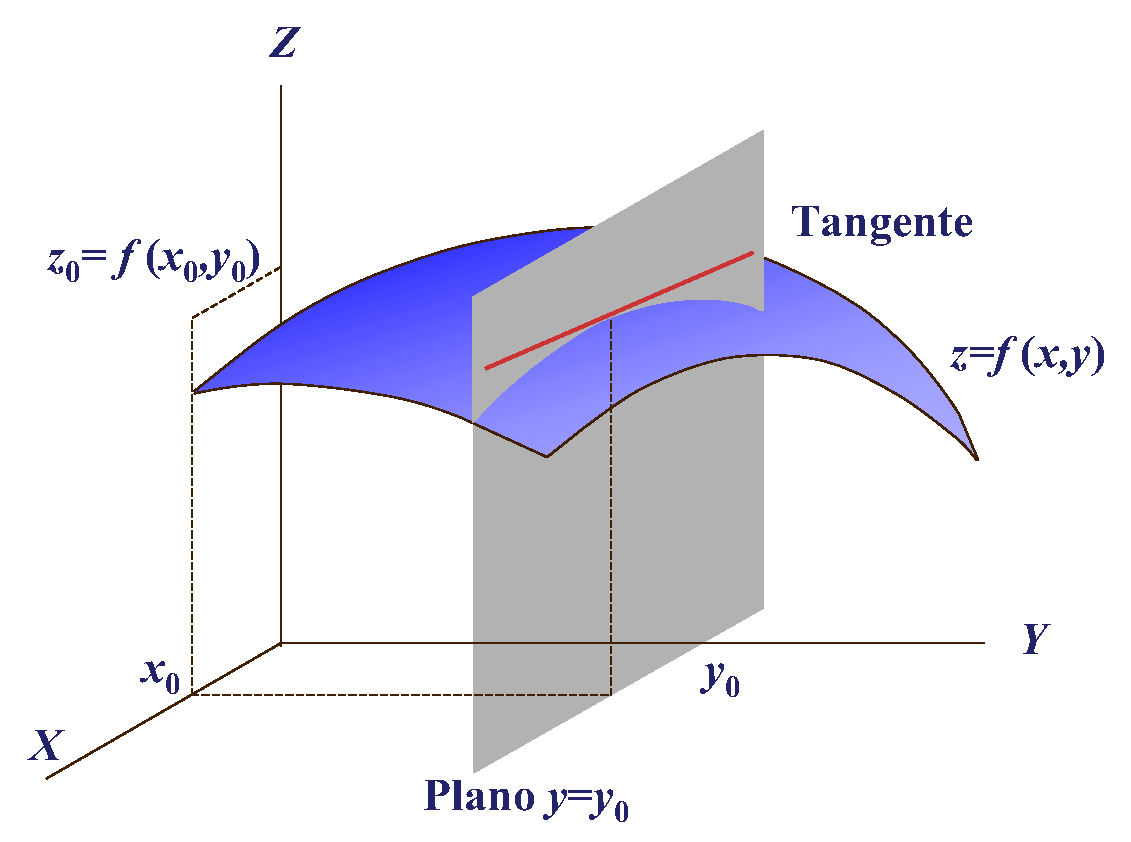
\includegraphics[scale=0.4]{img/tangentesuperficie}
\end{center}
\end{frame}


%---------------------------------------------------------------------slide----
\begin{frame}
\frametitle{Derivada parcial}
El concepto de derivada parcial visto para funciones de dos variables puede extenderse fácilmente para funciones de $n$ variables.

\begin{definicion}[Derivada parcial]
Dada una función de $n$ variables $f(x_1,\ldots,x_n)$, se dice que $f$ es \emph{derivable parcialmente} con respecto a la variable $x_i$ en el punto $a=(a_1,\ldots,a_n)$ si existe el límite
\[
\lim_{h\rightarrow 0} \frac{f(a_1,\ldots,a_{i-1},a_i+h,a_{i+1},\ldots,a_n)-f(a_1,\ldots,a_{i-1},a_i,a_{i+1},\ldots,a_n)} {h}.
\]
En tal caso, al valor del límite se le llama \emph{derivada parcial} de $f$ con respecto a la variable $x_i$, y se denota
\[
f'_{x_i}(a)=\frac{\partial f}{\partial x_i}(a).
\]
\end{definicion}
La definición de derivada para funciones de una variable es un caso particular de esta definición para $n=1$.
\end{frame}


%---------------------------------------------------------------------slide----
\begin{frame}
\frametitle{Cálculo de la derivada parcial}
Al medir la variación de $f$ con respecto a la variación de una sola de sus variables $x_i$ en un punto $a=(a_1,\ldots,a_n)$, el resto de las variables se pueden considerar como constantes y, en tal caso, podemos ver a $f$ como una función de una sola variable
\[
g(x_i)=f(a_1,\ldots,a_{i-1},x_i,a_{i+1},\ldots,a_n).
\]

La derivada parcial de $f$ con respecto a $x_i$ puede calcularse derivando esta función:
\[
\frac{\partial f}{\partial x_i}(a)=\frac{dg}{dx_i}(a_i)=g'(a_i).
\]

\begin{block}{Regla}
Para derivar parcialmente $f(x_1,\ldots,x_n)$ con respecto a una variable $x_i$, se deriva $f$ como si la única variable fuese $x_i$, tratando el resto de las variables como constantes.
\end{block} 
\end{frame}


%---------------------------------------------------------------------slide----
\begin{frame}
\frametitle{Cálculo de la derivada parcial}
\framesubtitle{Ejemplo con el volumen de un gas perfecto}
En la ecuación de los gases perfectos, el volumen es una función que depende de dos variables  
\[v(t,p)=\frac{nRt}{p},\]
donde $t$ mide la temperatura, $p$ la presión y $n$ y $R$ son constantes.

La tasa de variación instantánea que experimenta el volumen con respecto a la presión viene dada por la derivada parcial de $v$ con respecto a $p$.

Para calcular esta derivada parcial se fija $t$ como constante y se deriva $v$ como si la única variable fuese $p$:
\[
\frac{\partial v}{\partial p}(t,p)=\frac{d}{dp}\left(\frac{nRt}{p}\right)_{\mbox{\scriptsize $t=$cte}}=\frac{-nRt}{p^2}.
\]

Del mismo modo, la tasa de variación instantánea del volumen con respecto a la temperatura es:
\[
\frac{\partial v}{\partial t}(t,p)=\frac{d}{dt}\left(\frac{nRt}{p}\right)_{\mbox{\scriptsize$p=$cte}}=\frac{nR}{p}.
\]
\end{frame}



\subsection{Vector gradiente}
%---------------------------------------------------------------------slide----
\begin{frame}
\frametitle{Vector gradiente}
\begin{definicion}[Vector gradiente]
Dada una función de varias variables $f(x_1,\ldots,x_n)$, para la que existen todas sus derivadas parciales en un punto $a=(a_1,\ldots,a_n)$, se define el \emph{vector gradiente} de $f$ en $a$, y se nota $\nabla f(a)$, como el vector cuyas componentes son las $n$ derivadas parciales de $f$ en $a$, es decir, 
\[
\nabla f(a_1,\ldots,a_n)=\left(\frac{\partial f}{\partial x_1}(a),\ldots,\frac{\partial f}{\partial x_n}(a)\right).
\]
\end{definicion}

El vector gradiente en un punto dado tiene la misma magnitud y dirección que la velocidad máxima de variación de la
función en ese punto. 

De este modo, \alert{\emph{$\nabla f(a)$ indica la dirección de máximo crecimiento de $f$ en el punto $a$}}, mientras que $- \nabla f(a)$ indica la dirección de máximo decrecimiento.
\end{frame}



% ---------------------------------------------------------------------slide----
\begin{frame}
\frametitle{Cálculo del vector gradiente}
\framesubtitle{Ejemplo con una función de temperatura}
Al calentar una superficie la temperatura $t$ (en ºC) en cada punto $(x,y,z)$ (en mt) de dicha superficie viene dada por
la función:
\[ 
t(x,y,z)=\frac{x}{y}+z^2. 
\]
\emph{¿En qué dirección y con qué magnitud aumentará más rápidamente la temperatura en el punto $(2,1,1)$ de dicha superficie?}


La dirección en la que más rápidamente aumenta la temperatura nos la da el vector gradiente 
\[
\nabla t(x,y,z)=\left(\frac{\partial t}{\partial x}(x,y,z),\frac{\partial t}{\partial y}(x,y,z),\frac{\partial t}{\partial
z}(x,y,z)\right)=\left(\frac{1}{y},\frac{-x}{y^2},2z\right).
\]

En el punto $(2,1,1)$ dicha dirección será
\[
\nabla t(2,1,1)=\left(\frac{1}{1},\frac{-2}{1^2},2\cdot 1\right)=(1,-2,2),
\]
y su magnitud 
\[
|\nabla f(2,1,1)|=|\sqrt{1^2+(-2)^2+2^2}|=|\sqrt{9}|=3 \mbox{ ºC/mt}.
\]
\end{frame}


\subsection{Derivadas parciales de segundo orden}
%---------------------------------------------------------------------slide----
\begin{frame}
\frametitle{Derivadas parciales de segundo orden}
Las derivadas parciales de una función son, a su vez, funciones de varias variables que muchas veces pueden volverse a
derivar parcialmente con respecto a alguna de sus variables. 

Si una función $f(x_1,\ldots,x_n)$ tiene derivada parcial $f'_{x_i}(x_1,\ldots,x_n)$ con respecto a la variable $x_i$ en un conjunto $A$, entonces podemos derivar de nuevo parcialmente $f'_{x_i}$ con respecto a la variable $x_j$. Esta segunda derivada, cuando existe, se llama \emph{derivada parcial de segundo orden} de $f$ con respecto a las variables $x_i$ y $x_j$, y se nota
\[
\frac{\partial ^2 f}{\partial x_j \partial x_i}= \frac{\partial}{\partial x_j}\left(\frac{\partial f}{\partial x_i}\right).
\]

De forma análoga se definen las derivadas de orden superior.
\end{frame}


%---------------------------------------------------------------------slide----
\begin{frame}
\frametitle{Cálculo de las derivadas parciales de segundo orden}
La función de dos variables
\[f(x,y)=x^y\]
tiene cuatro derivadas parciales de segundo orden, que son:
\begin{align*}
\frac{\partial^2 f}{\partial x^2}(x,y) &=
\frac{\partial}{\partial x}\left(\frac{\partial f}{\partial x}(x,y)\right) =
\frac{\partial}{\partial x}\left(yx^{y-1}\right) =
y(y-1)x^{y-2},\\
\frac{\partial^2 f}{\partial y \partial x}(x,y) &=
\frac{\partial}{\partial y}\left(\frac{\partial f}{\partial x}(x,y)\right) =
\frac{\partial}{\partial y}\left(yx^{y-1}\right) =
x^{y-1}+yx^{y-1}\log x,\\
\frac{\partial^2 f}{\partial x \partial y}(x,y) &=
\frac{\partial}{\partial x}\left(\frac{\partial f}{\partial y}(x,y)\right) =
\frac{\partial}{\partial x}\left(x^y\log x \right) =
yx^{y-1}\log x+x^y\frac{1}{x},\\
\frac{\partial^2 f}{\partial y^2}(x,y) &=
\frac{\partial}{\partial y}\left(\frac{\partial f}{\partial y}(x,y)\right) =
\frac{\partial}{\partial y}\left(x^y\log x \right) =
x^y(\log x)^2.
\end{align*}
\end{frame}


\subsection{Matriz hessiana}
%---------------------------------------------------------------------slide----
\begin{frame}
\frametitle{Matriz hessiana y f hessiano}
\begin{definicion}[Matriz hessiana]
Dada una función de varias variables $f(x_1,\ldots,x_n)$, para la que existen todas sus derivadas parciales de segundo orden en un punto $a=(a_1,\ldots,a_n)$, se define la \emph{matriz hessiana} de $f$ en $a$, y se nota $Hf(a)$, como la matriz cuadrada cuyos elementos son 
\[
Hf(a)=\left(
\begin{array}{cccc}
\dfrac{\partial^2 f}{\partial x_1^2}(a) & 
\dfrac{\partial^2 f}{\partial x_1 \partial x_2}(a) &
\cdots &
\dfrac{\partial^2 f}{\partial x_1 \partial x_n}(a)\\
\dfrac{\partial^2 f}{\partial x_2 \partial x_1}(a) &
\dfrac{\partial^2 f}{\partial x_2^2}(a) & 
\cdots &
\dfrac{\partial^2 f}{\partial x_2 \partial x_n}(a)\\
\vdots & \vdots & \ddots & \vdots \\
\dfrac{\partial^2 f}{\partial x_n \partial x_1}(a) &
\dfrac{\partial^2 f}{\partial x_n \partial x_2}(a) &
\cdots &
\dfrac{\partial^2 f}{\partial x_n^2}(a)
\end{array}
\right).
\]
Al determinante de esta matriz se le llama \emph{hessiano} de $f$ en $a$.
\end{definicion}
\end{frame}


%---------------------------------------------------------------------slide----
\begin{frame}
\frametitle{Cálculo de la matriz hessiana y el hessiano}
Consideremos de nuevo la función de dos variables
\[f(x,y)=x^y.\]
Su matriz hessiana es:
\[
Hf(x,y)=\left(
\begin{array}{cc}
\dfrac{\partial^2 f}{\partial x^2} & \dfrac{\partial^2 f}{\partial x \partial y}\\
\dfrac{\partial^2 f}{\partial y \partial x} & \dfrac{\partial^2 f}{\partial y^2} 
\end{array}
\right)
=
\left(
\begin{array}{cc}
y(y-1)x^{y-2} & x^{y-1}(y\log x+1) \\
x^{y-1}(y\log x+1) & x^y(\log x)^2
\end{array}
\right).
\]

En el punto $(1,2)$ la matriz vale
\[
Hf(1,2)=\left(
\begin{array}{cc}
2(2-1)1^{2-2} & 1^{2-1}(2\log 1+1) \\
1^{2-1}(2\log 1+1) & 1^2(\log 1)^2
\end{array}
\right)
=
\left(
\begin{array}{cc}
2 & 1 \\
1 & 0 
\end{array}
\right).
\]

Y el hessiano en dicho punto vale
\[ |Hf(1,2)|=\left|
\begin{array}{cc}
2 & 1 \\
1 & 0
\end{array}
\right|=
2\cdot 0-1\cdot1= -1.\]
\end{frame}


%---------------------------------------------------------------------slide----
\begin{frame}
\frametitle{Igualdad de las derivadas cruzadas}
En el ejemplo anterior se aprecia que las \emph{derivadas cruzadas} de segundo orden $\frac{\partial^2 f}{\partial y\partial x}$ y $\frac{\partial^2 f}{\partial x\partial y}$ coinciden. Ello es debido al siguiente teorema: 

\begin{teorema}[Igualdad derivadas cruzadas]
Si $f(x,y)$ es una función tal que sus derivadas parciales $\frac{\partial f}{\partial x}$, $dfrac{\partial f}{\partial y}$, $dfrac{\partial^2 f}{\partial y\partial x}$ y $dfrac{\partial^2 f}{\partial x\partial y}$ existen y son continuas en un conjunto abierto $A$, entonces
\[
\frac{\partial^2 f}{\partial y\partial x}=\frac{\partial^2 f}{\partial x\partial y}.
\]
\end{teorema}

Una consecuencia del teorema es que, al calcular una derivada parcial de segundo orden que cumpla lo anterior, \alert{\emph{¡el orden en que se realicen las derivadas parciales no importa!}}

Si el teorema se cumple para todas las derivadas parciales de segundo orden, entonces la matriz hessiana es simétrica. 
\end{frame}
